\begin{figure}[p]
  \centering
  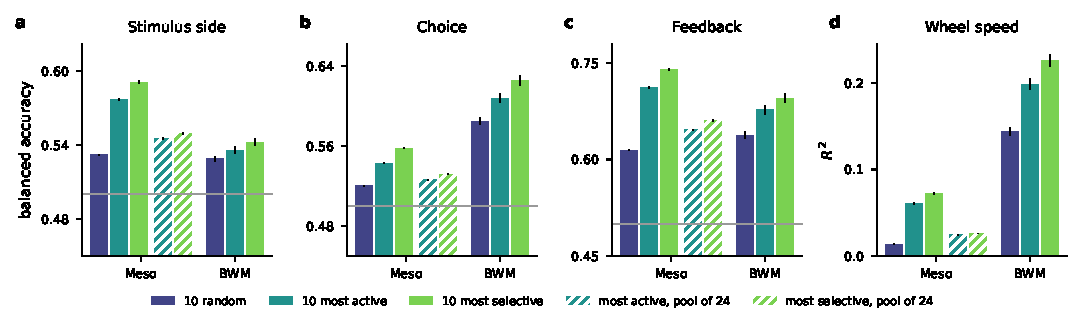
\includegraphics[width=7.00in,height=0.78\textheight,keepaspectratio]{si/si_selection_panels.pdf}
  \caption{Neuron selection. Decoding per session $\times$ bin (0.4\,mm bins, $\geq$10 neurons) from 10 neurons: randomly drawn (mean of 3 draws; as in the main figures), the 10 most active (highest fraction of non-zero window values; labels not used; a stand-in for ROI quality selection), or the 10 most selective for the decoded variable ($|$AUC$-0.5|$ for the binary variables, $|r|$ with wheel speed), selected separately in each outer cross-validation fold from its training trials only, so the test trials do not influence the selection (checked: shuffled labels give chance scores). Bars: mean $\pm$ s.e.m.\ over session $\times$ bin pairs. Selecting the most selective neurons raises mesoscope choice decoding from 0.520 to 0.558 (BWM 0.585 $\to$ 0.625), feedback from 0.614 to 0.740 (BWM 0.638 $\to$ 0.695) and wheel $R^2$ from 0.014 to 0.072 (BWM 0.144 $\to$ 0.226). Mesoscope bins hold more neurons per session than BWM bins (median 140 vs 24), which gives the selection more to choose from; hatched bars: the same selection from 24 randomly drawn neurons of the bin (pool size matched to the BWM median). With the matched pool, mesoscope scores are 0.549 / 0.532 / 0.660 and $R^2$ 0.026 (stimulus side / choice / feedback / wheel; most selective). \textbf{a} Stimulus side. \textbf{b} Choice. \textbf{c} Feedback. \textbf{d} Wheel speed ($R^2$).}
  \label{fig:si_selection}
\end{figure}
